花崗岩コアを伝播する弾性波を計測するため行った実験の方法について述べる。
以下でははじめに、実験に用いたコアサンプルについて、次に、強い弾性波を励起する
ために設計、制作した圧電超音波トランスデューサについて述べた後,計測システム全体の構成
と計測点の配置を示す。
\subsection{実験供試体}
超音波計測に用いた花崗岩供試体の外観と、形状および大きさを図\ref{fig:fig1}に示す。
供試体は、岡山県万成の採石場で採取した万成花崗岩を円柱状に加工したもので、直径は
約66mm, 高さは60mmである。主要造岩鉱物は石英、雲母、ナトリウムおよびカリ長石で。
数mmから数cm程度の結晶粒から構成される。外観からは肉眼で観察できるき裂などはなく、
風化もや造岩鉱物の明らかな変質も認められない。
ここで、供試体内部と表面の位置を指定するための$XYZ$直交座標を図\ref{fig:fig1}の
(b)および(c)のように取る。超音波の送信と受信は、供試体の上面$(Z=0)mm$で行い,
主として直径方向に伝播する表面波を観測する。
%--------------------
\begin{figure}[h]
	\begin{center}
	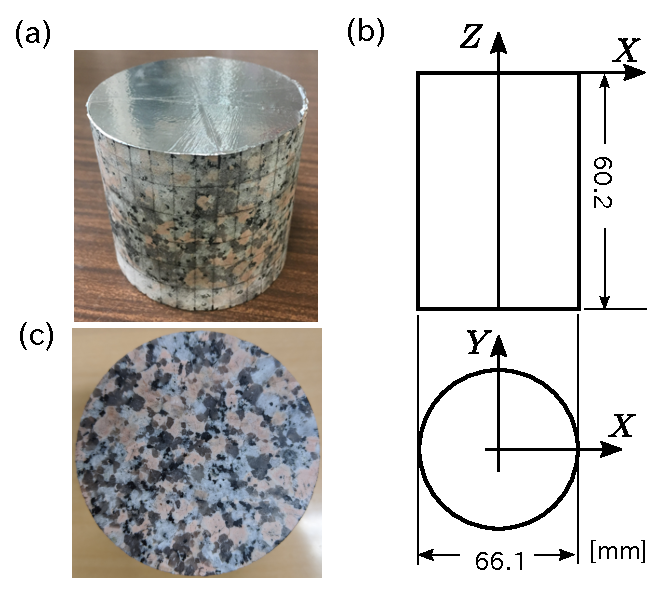
\includegraphics[width=0.6\linewidth]{Figs/fig1.eps} 
	\end{center}
	\caption{
		超音波計測に用いた花崗岩コア供試体(万成花崗岩).
	} 
	\label{fig:fig1}
\end{figure}
%--------------------
\subsection{送信超音波トランスデューサ}
本年度の実験のために、超音波を送信するためのトランューサを設計、制作した。
圧電超音波トランスデューサの構成を図\ref{fig:fig2}に示す。
曲率をもった圧電素子がくさび状のポリエーテルイミドのシューにマウントされている。
圧電素子の曲率中心はシューの先端部にある。
シュー先端部の幅は1mmで、圧電素子の周波数は2MHz.
花崗岩試料の弾性波速度は、縦波が約5km/s, 横波が3km/s程度であることがわかっている。
そのため、2MHzの超音波の岩石試料内部での波長は縦波。横波のそれぞれ、およそ2.5mm, 1.5mm程度となる。
試料表面の方向に十分な強度の超音波を送信するためには、シュー先端の幅は波長程度の寸法にする必要がある。
ここでは、先端部の幅を2MHzの横波波長よりも小さくなるよう、1mmとした。
圧電素子の幅は、シュー先端部の幅と岩石中での超音波の波長よりも十分に長くなるよう
40mmとした。これにより、線音源に近い状態を作り、平面波を励起する。
完全な平面波は距離による減衰が無く、伝播挙動を理解しやすい。
このことは、岩石のような強い散乱減衰を起こす、不均質材中の弾性波挙動を調べる上で重要である。





%--------------------
\begin{figure}[h]
	\begin{center}
	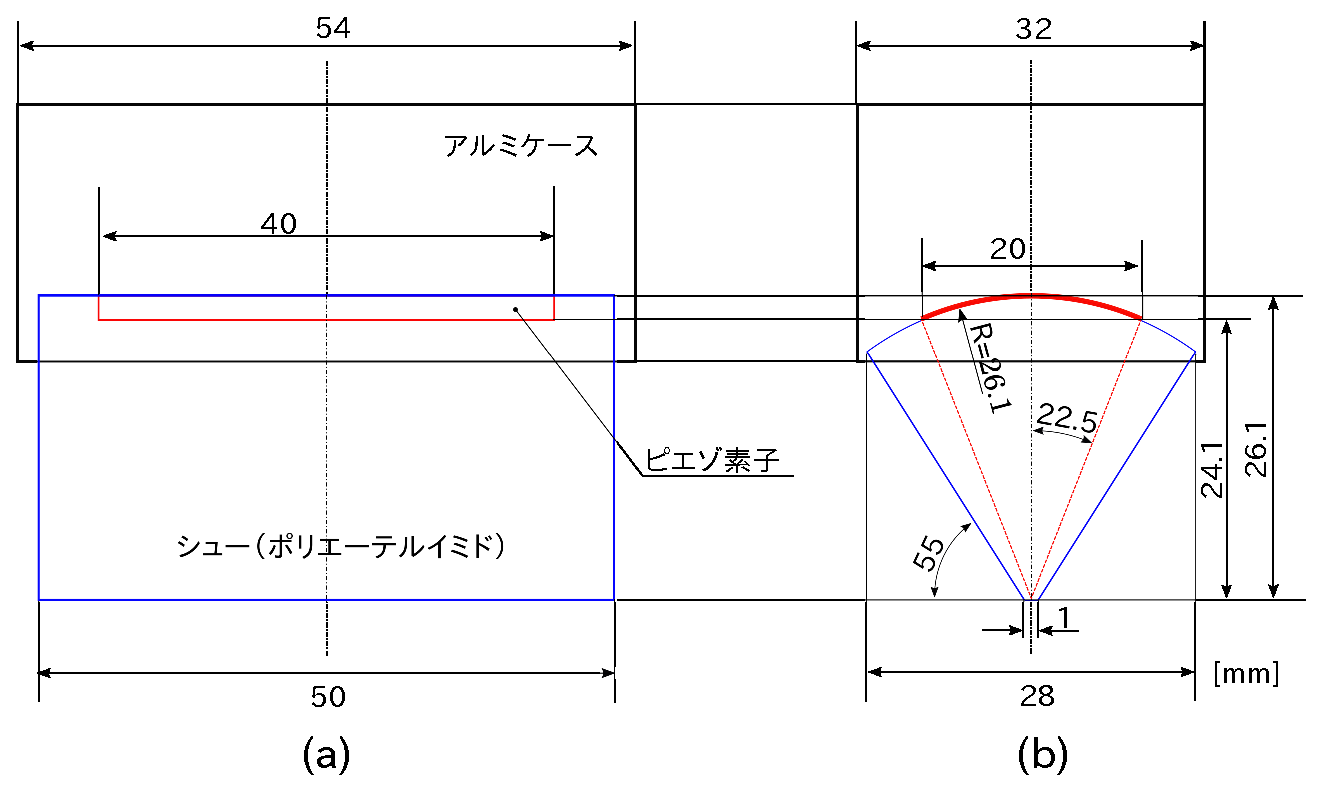
\includegraphics[width=0.8\linewidth]{Figs/fig2.eps} 
	\end{center}
	\caption{
		接触型ラインフォーカス探触子の形状と寸法.
	} 
	\label{fig:fig2}
\end{figure}
%--------------------
%--------------------
\begin{figure}[h]
	\begin{center}
	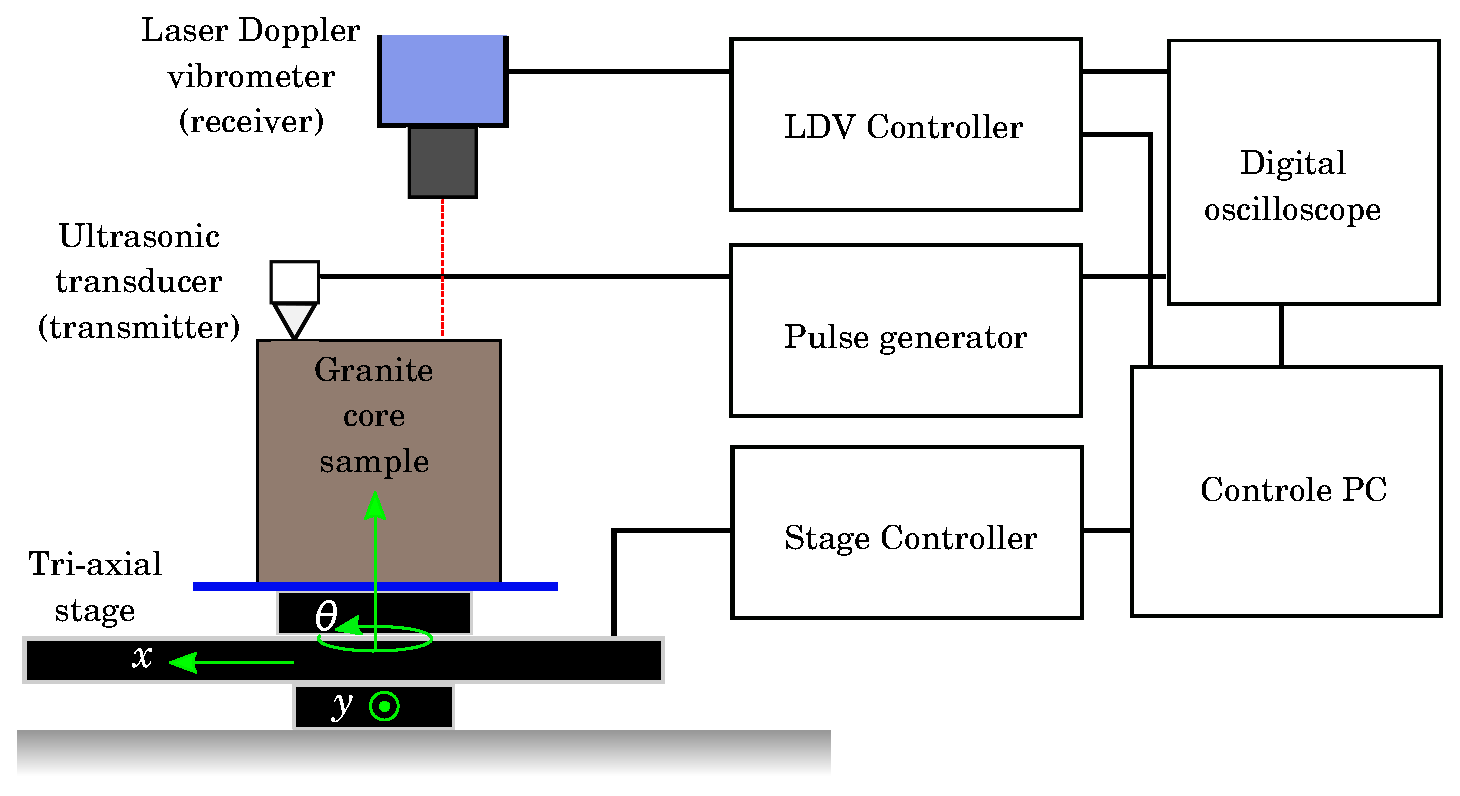
\includegraphics[width=0.8\linewidth]{Figs/fig3.eps} 
	\end{center}
	\caption{
		超音波測定装置の構成.
	} 
	\label{fig:fig3}
\end{figure}
%--------------------
%--------------------
\begin{figure}[h]
	\begin{center}
	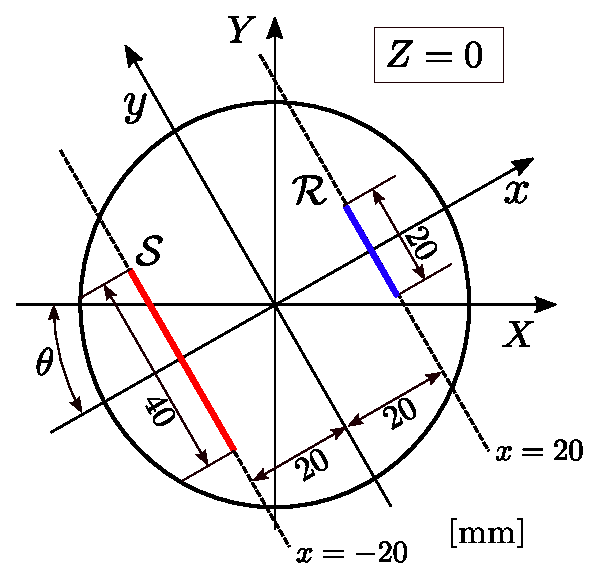
\includegraphics[width=0.5\linewidth]{Figs/fig4.eps} 
	\end{center}
	\caption{
		花崗岩コア供試体の上面における超音波送受信位置の配置.
		${\cal S}$は,ラインフォーカス探触子のカップリング位置を,
		${\cal R}$は,レーザー振動計による計測の測線を表す.
	} 
	\label{fig:fig4}
\end{figure}
%--------------------
%--------------------
\begin{figure}[h]
	\begin{center}
	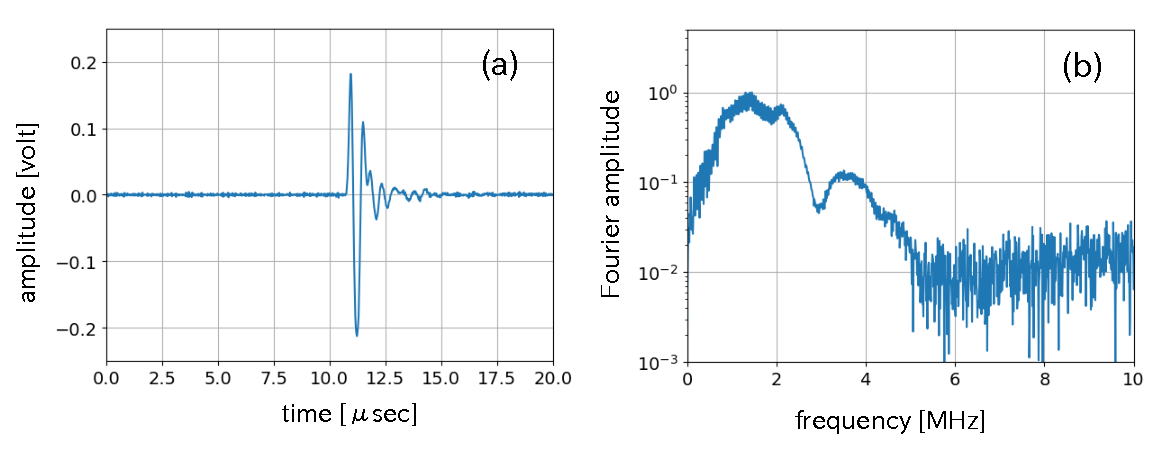
\includegraphics[width=0.9\linewidth]{Figs/fig5.eps} 
	\end{center}
	\caption{
		レーザードップラー振動計で計測した,ラインフォーカス探触子シュー先端部の振動速度波形.
	} 
	\label{fig:fig5}
\end{figure}
%--------------------
